Commuting sets of stabilizers enable the ability to detect different errors simultaneously without disturbing information. Finding such sets is non-trivial, and special codes have to be designed.

The general design principle behind the surface code is that the code is built up by patching repeated elements. This approach ensures that the surface code can be straightforwardly scaled whilst ensuring stabilizer commutativity. One advantage of the surface code is that it requires only nearest-neighbor interactions, as high-fidelity long-range interactions are difficult to maintain.

\subsubsection{The surface code four-cycle}

The basic element in the surface code is shown in the figure~\ref{fig:four_cycle} below, squares represent ancilla qubits, while circles represent data qubits. Black edges represent controlled $X$ gates, each controlled on an ancilla qubit $A$ and acting on a data qubit $D$. Likewise, the dashed edges represent controlled-$Z$ operations, each controlled by an ancilla qubit and acting on a data qubit.
For example, ancilla $A_1$ measures the stabilizer $XD_1XD_2$.
\begin{figure}[h]
    \centering
    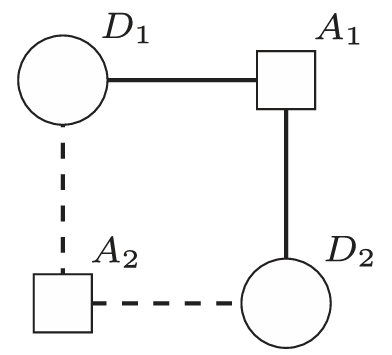
\includegraphics[width=0.2\textwidth]{sections/2_review_surface_code/four_cycle.png}
    \caption{Pictorial representation of the four cycle. The code qubits, $D_1$ and $D_2$, are represented by the circular nodes. The ancilla qubits, $A_1$ and $A_2$, are represented by the square nodes. The black and dashed edges depict controlled-$X$ and controlled-$Z$ operations controlled on the ancilla qubits and acting on the code qubits.}
    \label{fig:four_cycle}
\end{figure}
The surface code four-cycle is not useful itself as it encodes $k=n-m=0$ qubits, but working detection and correction codes can be formed by tiling together multiple four-cycles to form square lattices.

\subsubsection{The [[5, 1, 2]] surface code}

The figure~\ref{fig:512} below shows the five-qubit surface code formed by tiling four four-cycles in a square.
\begin{figure}[h]
    \centering
    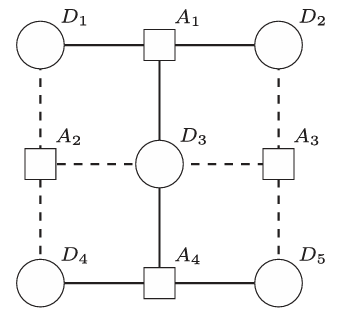
\includegraphics[width=0.2\textwidth]{sections/2_review_surface_code/512.png}
    \caption{The $[[5,1,2]]$ surface code is formed by tiling together four four-cycles in a square lattice.}
    \label{fig:512}
\end{figure}
The stabilizers can be read off to give

The logical operators of the surface code can be defined as chains of Pauli operators along the edges of the boundaries of the surface code. For example, $XD_1XD_4$ and $ZD_1ZD_2$ are both valid operators.

\begin{figure}[h]
    \centering
    \begin{minipage}{0.2\textwidth}
        \centering
        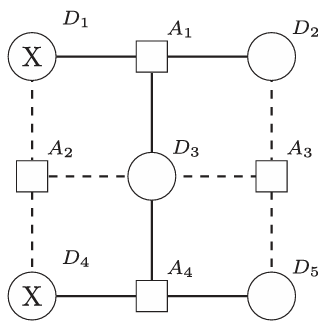
\includegraphics[width=\linewidth]{sections/2_review_surface_code/512-operators1.png}
        \caption*{(a)}
        \label{fig:image1}
    \end{minipage}
    \hspace{0.02\textwidth}
    \begin{minipage}{0.2\textwidth}
        \centering
        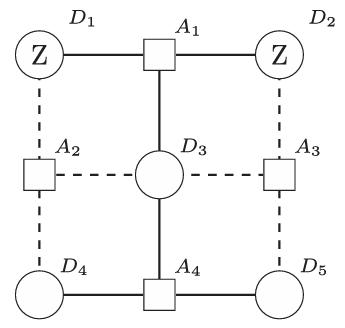
\includegraphics[width=\linewidth]{sections/2_review_surface_code/512-operators2.png}
        \caption*{(b)}
        \label{fig:image2}
    \end{minipage}
    \caption{The logical operators of a surface code can be defined as chains of Pauli operations that act along the boundaries of the lattice.}
    \label{fig:side_by_side_images}
\end{figure}
From the above we see that the minimum weight of the logical operators is 2, meaning the $[[5,1,2]]$ code is a detection code with $d=2$.

\subsubsection{Scaling}

The distance of a surface code can be increased simply by scaling the size of the lattice. The figure~\ref{fig:1313} shown below is the $[[13, 1, 3]]$ surface code, stabilizers and operators can be read off just by inspection.
\begin{figure}[h]
    \centering
    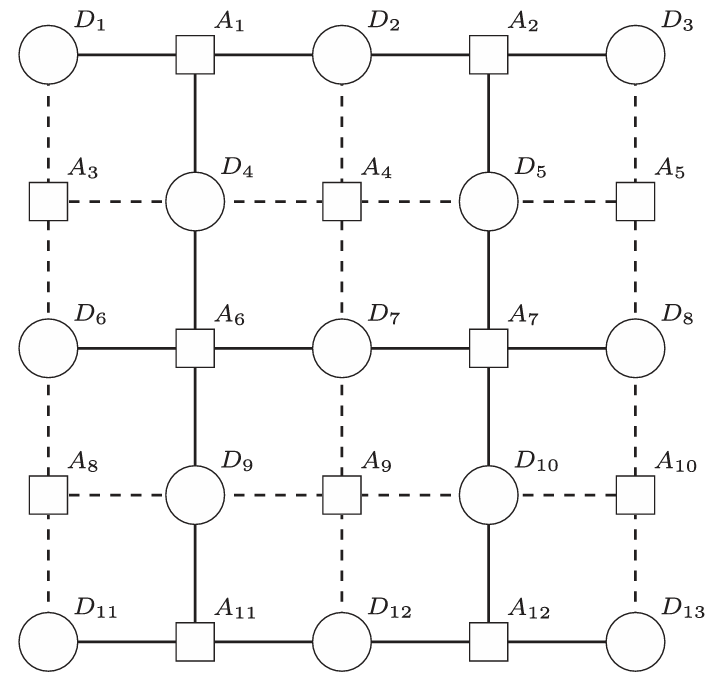
\includegraphics[width=0.2\textwidth]{sections/2_review_surface_code/1313.png}
    \caption{A distance-three surface code with parameters $[[13, 1, 3]]$.}
    \label{fig:1313}
\end{figure}